Như đã nói bên trên, khi biểu diễn mạng thần kinh nhân tạo dưới dạng đồ thị tính toán, để tính giá trị của một nút ta cần phải tính giá trị của tất cả các nút ở lớp trước đó. Ví dụ mạng thần kinh nhân tạo với mỗi lớp chỉ có duy nhất một nút, hàm để tính giá trị của nút ở lớp $m$ là $g(x)$, ở lớp $m+1$ là $f(x)$, nếu ta chọn $f(x)=g(x)$ là hàm sigmoid, thì giá trị của nút ở lớp $m+1$ là
\begin{align}
    f(g(x))=\dfrac{1}{1+\exp\left[-\dfrac{1}{1+\exp(-x)}\right]}
\end{align}
Nếu ta tiếp tục tăng số lớp lên, thì giá trị của nút ở lớp $m+n$ sẽ có dạng
\begin{align}
    f(\cdots z(x))=\dfrac{1}{1+\exp\left[-\dfrac{1}{1+\exp\left[-\cdots-\dfrac{1}{1+\exp(-x)}\right]}\right]}
    \label{equation:expansion-formula-nn}
\end{align}

Đối với các thuật toán học máy truyền thống, ta phải tìm hàm $\hat{y}=f(\mathbf{x},\mathbf{w})$, rồi ta chọn một hàm mất mát để đánh giá sai số giữa $\hat{y}$ và $y$. Hàm mất mát này sẽ có dạng $L=L(y,\hat{y})=L(y,\mathbf{x},\mathbf{w})$. Sau đó ta phải khai triển đại số và rút gọn $L$, rồi áp dụng thuật toán xuống đồi để tối ưu vector $\mathbf{w}$. Để đơn giản hoá, thay vì tính đạo hàm của hàm mất mát $L$, ta sẽ tính đạo hàm của $\hat{y}$, rồi từ đó suy ngược lại đạo hàm của $L(y,\hat{y})$. Đối với mạng thần kinh nhân tạo, việc tìm ra công thức rút gọn của $\hat{y}$ gần như là không thể vì nó thường là các hàm phi tuyến lồng vô nhau, nghĩa là công thức của hàm này sẽ rất dài và phức tạp (ví dụ trong hàm \ref{equation:expansion-formula-nn}) dẫn đến việc tính đạo hàm này sẽ trở nên khó khăn, và độ khó khăn sẽ tăng lên càng cao nếu như ta tăng số lượng lớp. Đây là vấn đề đầu tiên khi dùng phương pháp giải thuật toán học máy truyền thống để tối ưu mạng thần kinh nhân tạo.

Vấn đề thứ hai gặp phải là độ phức tạp sẽ tăng khi ta tăng số lượng nút trong lớp. Xét một mạng thần kinh có $n$ lớp, mỗi lớp có 2 nút, biểu diễn đồ thị tính toán ở hình \ref{figure:computational-graph-of-n-layer-2-node-nn}.
\begin{figure}[htb]
    \centering
    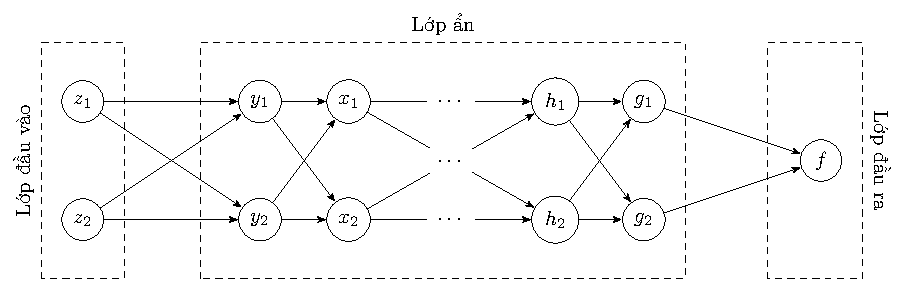
\includegraphics[width=0.8\textwidth]{tikz_image/complexity_graph.pdf}
    \caption{Mạng thần kinh với $n$ lớp, mỗi lớp có 2 nút}
    \label{figure:n-layer-2-node-nn}
\end{figure}
\begin{figure}[htb]
    \centering
    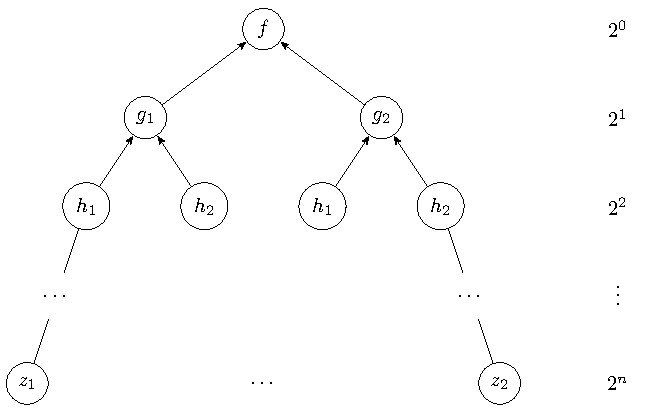
\includegraphics[width=0.5\textwidth]{tikz_image/complexity_tree.pdf}
    \caption{Đồ thị tính toán của mạng ở hình \ref{figure:n-layer-2-node-nn}}
    \label{figure:computational-graph-of-n-layer-2-node-nn}
\end{figure}

Nhìn đồ thị tính toán, để tìm công thức tổng quát của hàm $f$ dựa trên đầu vào $z_1,z_2$, ta phải khai triển các hàm lồng nhau. Ở tầng đầu tiên ta không có hàm lồng nhau nên số hàm lồng nhau phải khai triển là $2^0=1$, ở tầng thứ hai có một lớp lồng nhau là $f(g_1,g_2)$ nên số hàm phải khai triển là $2^1=2$, tương tự khi ta đi qua từng lớp đến đến lớp cuối cùng $n$, thì tổng số hàm lồng nhau mà ta phải khai triển là $2^n$. Độ phức tạp khi tính toán sẽ tăng theo cấp số nhân khi mà số lượng lớp tăng lên.

Để giải quyết vấn đề đầu tiên, nghĩa là không phải tính các hàm lồng nhau, người ta đưa ra giải pháp là áp dụng quy tắc xích (\textit{chain rule}) liên tục lặp đi lặp lại để tính đạo hàm ở từng lớp kế nhau (đạo hàm ở lớp $m$ đối với các nút ở lớp $m-1$), việc này làm giảm độ phức tạp vì chỉ phải tính đạo hàm trên một lớp duy nhất, không cần phải khai triển toàn bộ hàm. Bắt đầu tính đạo hàm ở lớp cuối cùng $n$, sau đó ta truyền giá trị đạo hàm xuống lớp kề nó (lớp $n-1$) để tính đạo hàm ở lớp này, rồi lặp lại quá trình này cho đến đầu đầu vào. Quá trình này gọi là lan truyền ngược, và việc tính toán theo cách số học (\textit{numerically}) cho từng lớp kế nhau sẽ dễ dàng hơn nhiều với việc tính toán kiểu đại số (\textit{algebraically}) trên toàn mạng rồi thay số vào.

Nhắc lại quy tắc xích
\begin{align}
    \dfrac{\partial f(g(x))}{\partial x} = \dfrac{\partial f(g(x))}{\partial g(x)}\cdot\dfrac{\partial g(x)}{\partial x}
\end{align}
\begin{figure}[htb]
    \centering
    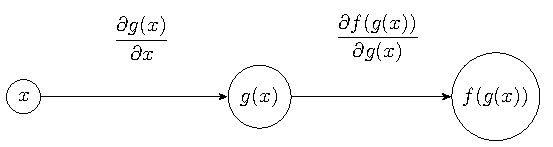
\includegraphics[width=0.5\textwidth]{tikz_image/chain_rule.pdf}
    \caption{Áp dụng quy tắc xích trong thần kinh đơn giản}
    \label{figure:chain-rule-nn}
\end{figure}
Đối với mạng thần kinh đơn giản (hình \ref{figure:chain-rule-nn}) với một nút đầu vào, một nút ẩn và một nút đầu ra, áp dụng quy tắc xích làm đơn giản hoá việc tính đạo hàm trên toàn mạng bằng việc tính đạo hàm trên từng cạnh rồi nhân với nhau. Đối với mạng thần kinh phức tạp hơn gồm nhiều lớp ẩn, mỗi lớp gồm nhiều nút, thì ta phải áp dụng quy tắc xích đa biến (\textit{multivariate chain rule})
\begin{align}
    \dfrac{\partial f(g_1(x),\dots,g_k(x))}{\partial x} = \sum^k_{i=1}\dfrac{\partial f(g_1(x),\dots,g_k(x))}{\partial g_i(x)}\cdot\dfrac{\partial g_i(x)}{\partial x}
\end{align}
Áp dụng quy tắc xích đa biến vào mạng (hình \ref{figure:multivariate-chain-rule-nn}), ta được
\begin{align}
    \label{equation:multivariate-chain-rule-nn}
    \dfrac{\partial o}{\partial x}=
    \dfrac{\partial f(g_1,g_2)}{\partial g_1}\cdot\dfrac{\partial g_1(h)}{\partial h}\cdot\dfrac{\partial h(x)}{\partial x}
    +\dfrac{\partial f(g_1,g_2)}{\partial g_2}\cdot\dfrac{\partial g_2(h)}{\partial h}\cdot\dfrac{\partial h(x)}{\partial x}
\end{align}
\begin{figure}[htb]
    \centering
    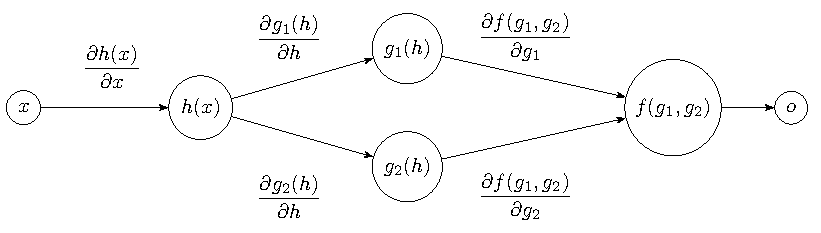
\includegraphics[width=0.8\textwidth]{tikz_image/multivariate_chain_rule.pdf}
    \caption{Áp dụng quy tắc xích đa biến trong mạng thần kinh phức tạp}
    \label{figure:multivariate-chain-rule-nn}
\end{figure}

Dựa vào quy tắc xích đa biến, Charu C. Aggarwal đã nêu ra bổ đề về tổng hợp của các cạnh (\textit{pathwise aggregation lemma}) \cite{Aggarwal2023-zk} như sau: gọi $y(i)$ là giá trị của nút $i$ trong mạng, gọi $z(i,j)=\partial y(j)/\partial y(i)$ là đạo hàm của cạnh $(i,j)$, gọi tập hợp các đường đi khác nhau xuất phát từ điểm $s$ và kết thúc ở điểm $t$ là $\mathcal{P}$, giá trị của đào hàm $\partial y(t)/\partial y(s)$ được tính bằng tích của các cạnh nối từ $s$ đến $t$, rồi lấy tổng theo các đường đi khác nhau dẫn từ $s$ đến $t$
\begin{align}
    \dfrac{\partial y(t)}{\partial y(s)}=\sum_{P\in\mathcal{P}}\ \prod_{(i,j)\in P}z(i,j)
    \label{equation:pathwise-aggregation-lemma}
\end{align}
Giải pháp này chỉ giải quyết được vấn đề đầu tiên mà không giải quyết được vấn đề thứ hai. Trong ví dụ hình \ref{figure:multivariate-chain-rule-nn}, có 2 con đường dẫn từ đầu vào đến đầu ra. Hai con đường này đều đi qua điểm $h(x)$, nên trong đạo hàm của hàm \ref{equation:multivariate-chain-rule-nn}, ta thấy có sự xuất hiện 2 lần của đạo hàm $\partial h(x)/\partial x$, nghĩa là nếu một cạnh $(i,j)$ xuất hiện trong $n$ đường đi ${P_1,\dots,P_n}\in\mathcal{P}$, thì ta phải tính đạo hàm của cạnh $(i,j)$ $n$ lần. Để giải quyết vấn đề tính trùng nhau này, người ta dùng phương pháp quy hoạch động (\textit{dynamic programming}) trong lý thuyết đồ thị (\textit{graph theory}).

Gọi $S(i,j)=\partial y(j)/\partial y(i)$, ta viết lại bổ đề \ref{equation:pathwise-aggregation-lemma} thành
\begin{align}
    S(s,t)=\sum_{P\in\mathcal{P}}\ \prod_{(i,j)\in P}z(i,j)
\end{align}
Chọn điểm $i$ bất kỳ trong mạng, gọi $j\in A(i)$ là tập hợp các điểm mà $i$ kết nối đến. Nếu tất cả giá trị của điểm $S(j,t)$ đã được tính, thì ta có hàm cập nhật $S(i,t)$ dựa trên các giá trị đã tính $S(j,t)$ là
\begin{align}
    S(i,t)=\sum_{j\in A(i)}z(i,j)S(j,t)
\end{align}
Với giá trị khởi tạo $S(t,t)=1$, mã giả của thuật toán quy hoạch động để tính $S(s,t)$ là
\begin{algorithmz}
    \caption{Mã giả tính $S(s,t)$ bằng quy hoạch động \cite{Aggarwal2023-zk}}
    \label{algorithm:dynamic-programming-node-to-node}
    \begin{algorithmic}[1]
        \State Khởi tạo $S(t,t)=1$
        \Repeat
        \State Chọn nút $i$ thoả tất cả giá trị $S(j,t)$ đã được tính, với $j\in A(i)$
        \State Cập nhật $S(i,t)\gets\sum_{j\in A(i)}z(i,j)S(j,t)$
        \Until tất cả các nút đã được tính
    \end{algorithmic}
\end{algorithmz}

Trong hầu hết các thuật toán học máy truyền thống, người ta chỉ cần tìm lời giải một lần duy nhất là một hàm $f$ dưới dạng rút gọn, sau đó chỉ cần thay các điểm dữ liệu khác nhau là ta sẽ cập nhật được bộ tham số $\mathbf{w}$ dựa theo thuật toán xuống đồi. Đối với thuật toán lan truyền ngược, ta phải chạy lại thuật toán với mỗi điểm khác nhau. Điều này nghe như khối lượng công việc sẽ nhiều hơn so với các thuật toán truyền thống, nhưng nó đã được chứng minh là tốt hơn nhiều so với cách giải truyền thống khi mà số lượng lớp và nút ở mỗi lớp lớn.

Như đã nói ở trên, sau khi đã tính được đạo hàm của $\partial y(j)/\partial y(i)$, ta phải suy ra đạo hàm của $\partial L/\partial\mathbf{w}$. Nếu mạng thần kinh có $p$ nút đầu ra, thì các nút đầu ra sẽ là $t_1,t_2,\dots,t_p$, hàm mất mát bây giờ sẽ là $L(y(t_1),y(t_2),\dots,y(t_p))$. Gọi $w_{ji}$ là tham số cạnh giữa hai nút $j$ và $i$. Khi này đạo hàm riêng của hàm mất mát sẽ là
\begin{align}
    \dfrac{\partial L}{\partial w_{ji}} & =
    \dfrac{\partial L}{\partial y(i)}\cdot\dfrac{\partial y(i)}{\partial w_{ji}\label{equation:loss-to-weight}}                                                                                                          \\
                                        & =\left[\sum^p_{k=1}\dfrac{\partial L}{\partial y(t_k)}\cdot\dfrac{\partial y(t_k)}{\partial y(i)}\right]\dfrac{\partial y(i)}{\partial w_{ji}}\label{equation:loss-to-weight1}
\end{align}
Giá trị của $\partial y(i)/\partial w_{ji}$ ($j$ là điểm nối đến $i$) có thể được tính theo hình \ref{figure:single-layer-network}. Giá trị của $\partial y(t_k)/\partial y(i)$ được tính bằng thuật toán quy hoạch động bên trên. Giá trị của $\partial L/\partial y(t_k)$ được tính như các thuật toán học máy truyền thống vì $L=L(y(t_1),y(t_2),\dots,y(t_p))$. Nhưng thay vì dùng thuật toán \ref{algorithm:dynamic-programming-node-to-node} để tính từng phần của \ref{equation:loss-to-weight1}, ta có thể biến đổi thuật toán này để tính $\partial L/\partial y(i)$.

Chọn điểm $i$ bất kỳ trong mạng, gọi $j\in A(i)$ là tập hợp các điểm mà $i$ kết nối đến. Đặt $\triangle(i)=\partial L/\partial y(i)$, dựa vào \ref{equation:loss-to-weight1}, ta có thể tính $\triangle(i)$ dựa trên các giá trị đã tính $\triangle(j)$
\begin{align}
    \triangle(i)=\sum_{j\in A(i)}z(i,j)\triangle(j)
\end{align}
Khởi tạo đạo hàm mất mát với tất cả các nút đầu ra $\triangle(t_k)$, ta có
\begin{algorithmz}
    \caption{Mã giả tính $\partial L/\partial\mathbf{w}$ bằng quy hoạch động \cite{Aggarwal2023-zk}}
    \label{algorithm:dynamic-programming-loss-to-weight}
    \begin{algorithmic}[1]
        \State Khởi tạo $\triangle(t_k)=\dfrac{\partial L}{\partial y(t_k)}$ với mỗi $k\in\{1,\dots,p\}$
        \Repeat
        \State Chọn nút $i$ thoả tất cả giá trị $\triangle(j)$ đã được tính, với $j\in A(i)$
        \State Cập nhật $\triangle(i)\gets\sum_{j\in A(i)}z(i,j)\triangle(j)$
        \Until tất cả các nút đã được tính
        \ForEach {cạnh $(j,i)$ có hệ số $w_{ji}$}
        \State Tính $\dfrac{\partial L}{\partial w_{ji}}\gets\triangle(i)\cdot\dfrac{\partial y(i)}{\partial w_{ji}}$
        \EndFor
    \end{algorithmic}
\end{algorithmz}\\
Sau khi tính $\partial L/\partial\mathbf{w}$, ta có thể áp dụng thuật toán xuống đồi để tối ưu tham số $\mathbf{w}$
\begin{align}
    \mathbf{w}\leftarrow\mathbf{w}-\alpha\cdot\dfrac{\partial L}{\partial\mathbf{w}}
\end{align}

Thuật toán \ref{algorithm:dynamic-programming-loss-to-weight} chỉ có thể áp dụng trong mạng thần kinh nhân tạo không có hàm kích hoạt. Gọi $B(i)$ là các nút kết nối đến nút $i$, $A(i)$ là các nút mà $i$ kết nối đến. Giá trị của nút trước khi qua hàm kích hoạt là $a(i)$, sau khi qua hàm kich hoạt là $h(i)=\Phi_i=\Phi(a(i))$. Khai triển của nút $i$ sẽ là một hàm tuyến tính các nút nối đến nó $a(i)=\sum_{j\in B(i)}w_{ji}h(j)$. Khi sử dụng hàm kích hoạt, ta phải biến đổi thuật toán theo một trong hai cách sau:
\begin{enumerate}
    \item Cách đầu tiên là sử dụng giá trị sau khi kích hoạt (\textit{post-activation}). Nếu ta đặt giá trị của nút $i$ là $y(i)=h(i)=\Phi(a(i))$ (giá trị sau hàm kích hoạt), thì trong thuật toán \ref{algorithm:dynamic-programming-loss-to-weight}, ta phải chú ý
          \begin{itemize}
              \item Giá trị $z(i,j)_{j\in A(i)}=\dfrac{\partial y(j)}{\partial y(i)}$ thay đổi thành
                    \begin{align}
                        z(i,j)
                         & =\dfrac{\partial\Phi(a(j))}{\partial\Phi(a(i))}                                          \nonumber \\
                         & =\dfrac{\partial\Phi(a(j))}{\partial a(j)}\cdot\dfrac{\partial a(j)}{\partial\Phi(a(i))} \nonumber \\
                         & =\Phi'_j\cdot w_{ij}
                    \end{align}
                    nên $\triangle(i)\gets\sum_{j\in A(i)}\left[\Phi'_j\cdot w_{ij}\right]\triangle(j)$
              \item Thay đổi
                    \begin{align}
                        \left[\dfrac{\partial y(i)}{\partial w_{ji}}\right]_{j\in B(i)}=\dfrac{\partial\Phi(a(i))}{\partial w_{ji}}=\dfrac{\partial\Phi(a(i))}{\partial a(i)}\cdot\dfrac{\partial a(i)}{w_{ji}}=\Phi'_i\cdot\Phi_j
                    \end{align}
                    nên $\dfrac{\partial L}{\partial w_{ji}}\gets\triangle(i)\left[\Phi'_i\cdot\Phi_j\right]$
          \end{itemize}
    \item Cách thứ hai là sử dụng giá trị trước khi kích hoạt (\textit{pre-activation}). Nếu ta đặt giá trị của nút $i$ là $y(i)=a(i)$ (giá trị trước hàm kích hoạt), thì mỗi khi tính giá trị $a(i)$ từ $a(j),j\in B(i)$, ta phải dùng hàm kích hoạt lên các giá trị đầu vào này $y(i)=a(i)=\sum_{j\in B(i)}\Phi(a(j))$. Lưu ý, vì ta chọn cách biến đổi $y(i)=a(i)$ nên ở lớp ẩn đầu tiên ta sẽ không phải tính hàm kích hoạt, và ở lớp đầu ra ta phải dùng hàm kích hoạt lên lớp này rồi mới đưa kết quả vào hàm mất mát.
          \begin{itemize}
              \item Giá trị khởi tạo sẽ là
                    \begin{align}
                        \dfrac{\partial L}{\partial y(t_r)}
                         & =\dfrac{\partial L}{\partial a(t_r)}                                                        \nonumber \\
                         & =\dfrac{\partial L}{\partial\Phi(a(t_r))}\cdot\dfrac{\partial\Phi(a(t_r))}{\partial a(t_r)} \nonumber \\
                         & =L'(\Phi_{t_r})\cdot\Phi'_{t_r}
                    \end{align}
                    % nên $\
              \item Tương tự như trên, giá trị $z(i,j)_{j\in A(i)}$ thay đổi thành
                    \begin{align}
                        z(i,j)
                         & =\dfrac{\partial a(j)}{\partial a(i)}                                                    \nonumber \\
                         & =\dfrac{\partial a(j)}{\partial\Phi(a(i))}\cdot\dfrac{\partial\Phi(a(i))}{\partial a(i)} \nonumber \\
                         & =w_{ij}\cdot\Phi'_i
                    \end{align}
                    nên $\triangle(i)\gets\Phi'_i\sum_{j\in A(i)}w_{ij}\cdot\triangle(j)$
              \item Thay đổi
                    \begin{align}
                        \left[\dfrac{\partial y(i)}{\partial w_{ji}}\right]_{j\in B(i)}=\dfrac{\partial a(i)}{\partial w_{ji}}=\Phi_j
                    \end{align}
                    nên $\dfrac{\partial L}{\partial w_{ji}}\gets\triangle(i)\cdot\Phi_j$
          \end{itemize}
\end{enumerate}

Cả hai cách trên đều được dùng trong mạng thần kinh nhân tạo, nhưng cách sử dụng giá trị trước khi kích hoạt thường được dùng nhiều hơn. Một số đạo hàm của hàm kích hoạt $\Phi'$ ở hình \ref{figure:differential-activation-funtion}.
\begin{figure}[htbp]
    \centering
    \begin{subfigure}[b]{0.33\textwidth}
        \centering
        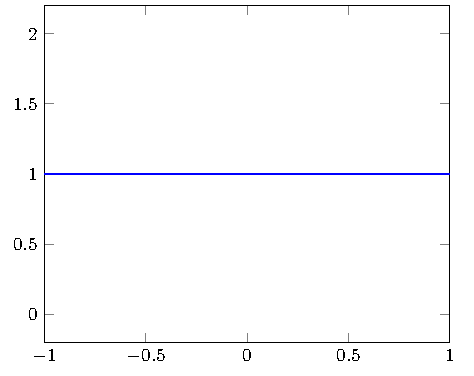
\includegraphics[width=\textwidth]{tikz_image/diff_identity.pdf}
        \caption{Hàm tuyến tính}
    \end{subfigure}%
    \begin{subfigure}[b]{0.33\textwidth}
        \centering
        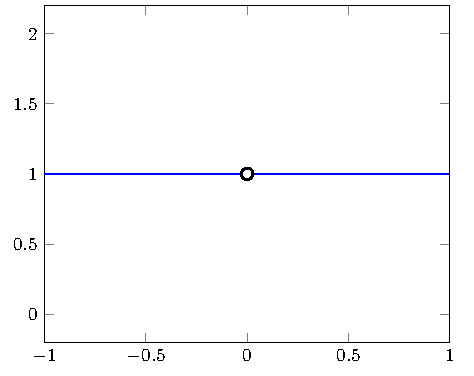
\includegraphics[width=\textwidth]{tikz_image/diff_sign.pdf}
        \caption{Hàm sign}
    \end{subfigure}%
    \begin{subfigure}[b]{0.33\textwidth}
        \centering
        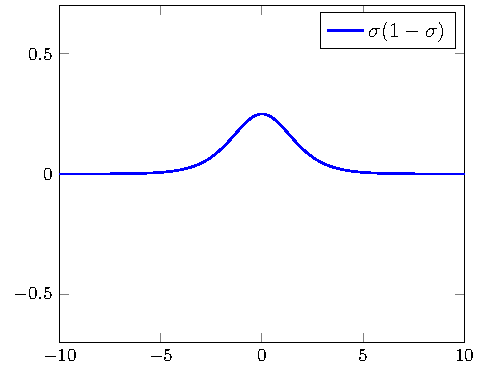
\includegraphics[width=\textwidth]{tikz_image/diff_sigmoid.pdf}
        \caption{Hàm sigmoid}
    \end{subfigure}\newline
    \begin{subfigure}[b]{0.33\textwidth}
        \centering
        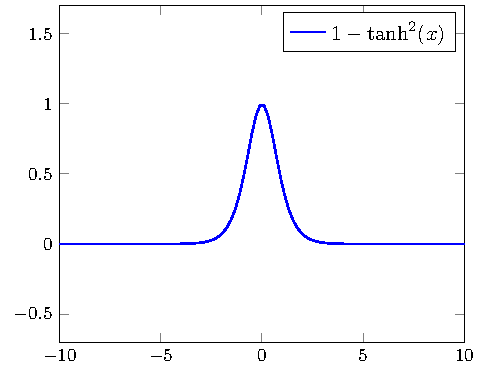
\includegraphics[width=\textwidth]{tikz_image/diff_tanh.pdf}
        \caption{Hàm tanh}
    \end{subfigure}%
    \begin{subfigure}[b]{0.33\textwidth}
        \centering
        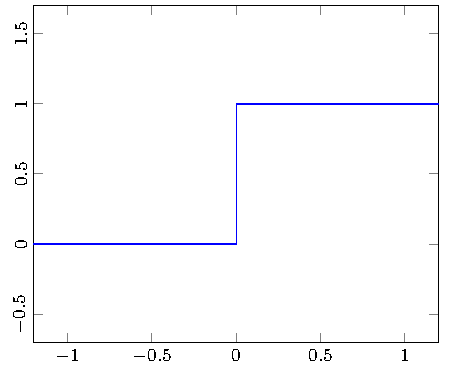
\includegraphics[width=\textwidth]{tikz_image/diff_relu.pdf}
        \caption{Hàm ReLu}
    \end{subfigure}%
    \begin{subfigure}[b]{0.33\textwidth}
        \centering
        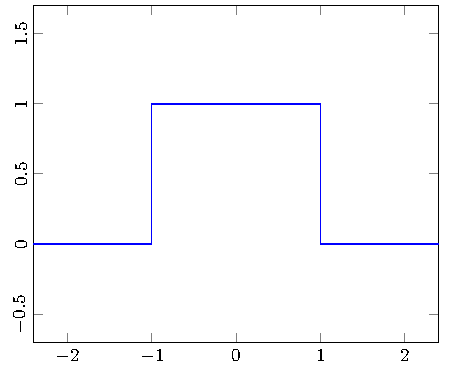
\includegraphics[width=\textwidth]{tikz_image/diff_hardtanh.pdf}
        \caption{Hàm hardtanh}
    \end{subfigure}%
    \caption{Đồ thị đạo hàm các hàm kích hoạt thông dụng}
    \label{figure:differential-activation-funtion}
\end{figure}

Đối với hàm kích hoạt softmax ở lớp đầu ra, ta không thể dùng thuật toán trên được mà phải thay đổi một chút ở lớp đầu ra khi đi qua hàm softmax. Gọi $o_1,\dots,o_p$ là giá trị xác suất của các biến đầu ra $t_1,\dots,t_p$, hàm softmax sẽ là
\begin{align}
    o_i=\dfrac{\exp(t_i)}{\sum_{j=1}^k\exp(t_j)}
\end{align}
Hàm softmax ở lớp đầu ra thường đi chung với hàm mất mát cross-entropy
\begin{align}
    L=-\sum_{i=1}^k y_i\log(o_i)
\end{align}
với $y_i$ là mã hoá one-hot của giá trị quan sát. Đạo hàm của hàm mất mát là
\begin{align}
    \label{equation:softmax-derivative}
    \dfrac{\partial L}{\partial t_i}
    =\sum_{j=1}^k\dfrac{\partial L}{\partial o_j}\cdot\dfrac{\partial o_j}{\partial t_i}
\end{align}
Với đạo hàm của hàm mất mát được tính theo mỗi đầu ra $o_j$
\begin{align}
    \dfrac{\partial L}{\partial o_j}=\dfrac{\partial[-y_j\log(o_j)]}{\partial o_j}=-\dfrac{y_j}{o_j}
\end{align}

Với hàm chỉ thị (\textit{indicator function}) $I(i,j)$, đạo hàm của giá trị sau và trước lớp softmax được tính bằng cách: \cite{webpage3}
\begin{align}
    \dfrac{\partial\log(o_j)}{\partial t_i}           & =\dfrac{1}{o_j}\cdot\dfrac{\partial o_j}{\partial t_i}                                                                                  \\
    \Leftrightarrow\dfrac{\partial o_j}{\partial t_i} & =o_j\cdot\dfrac{\partial\log(o_j)}{\partial t_i}
    =o_j\cdot\dfrac{\partial}{\partial t_i}\log\left[\dfrac{\exp(t_j)}{\sum_{l=1}^k\exp(t_l)}\right]                                                                                  \nonumber \\
                                                      & =o_j\cdot\left[\dfrac{\partial t_j}{\partial t_i}-\dfrac{\partial}{\partial t_i}\log\left[\sum_{l=1}^k\exp(t_l)\right]\right] \nonumber \\
                                                      & =o_j\cdot\left[\dfrac{\partial t_j}{\partial t_i}-\dfrac{\exp(t_i)}{\sum_{l=1}^k\exp(t_l)}\right]                             \nonumber \\
                                                      & =o_j\cdot(I(i,j)-o_i)
\end{align}
Thay vào phương trình \ref{equation:softmax-derivative}, ta có
\begin{align}
    \dfrac{\partial L}{\partial t_i}
     & =\sum_{j=1}^k-\dfrac{y_j}{o_j}\cdot o_j\cdot(I(i,j)-o_i) \nonumber \\
     & =o_i\sum_{j=1}^k y_j-\sum_{j=1}^k I(i,j)y_j              \nonumber \\
     & =o_i-y_i
\end{align}

Thuật toán \ref{algorithm:dynamic-programming-loss-to-weight} sau khi sửa đổi để sử dụng với hàm kích hoạt $\Phi$ là hoàn chỉnh để lập trình mạng thần kinh nhân tạo trên máy tính. Tuy nhiên thuật toán này không sử dụng các tính toán trên ma trận nên không thể tận dụng được sức mạnh phần cứng của GPU hay các thiết bị XLA. Vì thế ta cần thay đổi thuật toán về dạng ma trận (phương trình \ref{equation:matrix-form}) để tối ưu sức mạnh tính toán.

Ta quy ước đạo hàm đối với một vector sẽ được viết dưới dạng ma trận sắp xếp theo mẫu số (\textit{denominator layout}). Ví dụ ta có hai vector cột $\textbf{h}$ và $\textbf{x}$, ma trận của đạo hàm là
\begin{align}
    \left[\dfrac{\partial\mathbf{h}}{\partial\mathbf{x}}\right]_{ij}=\dfrac{\partial h_j}{\partial x_i}
\end{align}
Ma trận này chính là ma trận Jacobi chuyển vị $\left[\dfrac{\partial\mathbf{h}}{\partial\mathbf{x}}\right]=J(\mathbf{h},\mathbf{x})^\intercal$.

Nếu $\mathbf{o}=F_k(F_{k-1}(\dots F_1(\mathbf{x})))$, với đầu vô của hàm $F_i$ có chiều là $n_i$, đầu ra của hàm $F_i$ có chiều là $n_{i+1}$, thì quy tắc xích khi viết dưới dạng ma trận sắp xếp theo mẫu số sẽ là
\begin{align}
    \underbrace{\left[\dfrac{\partial\mathbf o}{\partial\mathbf x}\right]}_{n_1\times n_{k+1}}=
    \underbrace{\left[\dfrac{\partial\mathbf h_1}{\partial\mathbf x}\right]}_{n_1\times n_2}
    \underbrace{\left[\dfrac{\partial\mathbf h_2}{\partial\mathbf h_1}\right]}_{n_2\times n_3}\cdots
    \underbrace{\left[\dfrac{\partial\mathbf h_{k-1}}{\partial\mathbf h_{k-2}}\right]}_{n_{k-1}\times n_k}
    \underbrace{\left[\dfrac{\partial\mathbf h_k}{\partial\mathbf h_{k-1}}\right]}_{n_k\times n_{k+1}}
\end{align}
Quy tắc xích này có thứ tự đảo ngược so với quy tắc xích bình thường vì ta đang quy ước ma trận của đạo hàm sẽ dưới dạng sắp xếp theo mẫu số.

Mỗi nút trong mạng thần kinh nhân tạo sẽ được tính qua hai bước là bước tổng tuyến tính và bước sử dụng hàm kích hoạt, nên ta sẽ chia mỗi lớp trong mạng thành hai lớp riêng biệt, lớp đầu tiên là lớp tuyến tính (phương trình \ref{equation:matrix-form}), sau đó là lớp kích hoạt (hình \ref{figure:multi-layer-linear-activation-matrix}).
\begin{figure}[htb]
    \centering
    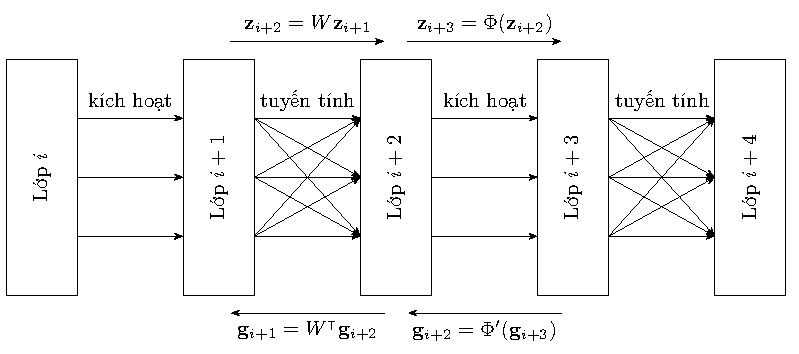
\includegraphics[width=0.8\textwidth]{tikz_image/multi_layer_linear_activation_matrix.pdf}
    \caption{Hai lớp tuyến tính và kích hoạt nằm xen kẽ nhau}
    \label{figure:multi-layer-linear-activation-matrix}
\end{figure}

Gọi $\mathbf z_i$ là vector giá trị của lớp $i$, $\mathbf g_i$ là vector đạo hàm $[\partial L/\partial\mathbf z_i]$, ta có
\begin{align}
     & \mathbf z_{i+1}=W\mathbf z_i                                                                      & \text{[Lan truyền xuôi ở lớp tuyến tính]} \\
     & \mathbf z_{i+1}=\Phi(\mathbf z_i)                                                                 & \text{[Lan truyền xuôi ở lớp kích hoạt]}  \\
     & \mathbf g_i=\left[\dfrac{\partial\mathbf z_{i+1}}{\partial\mathbf z_i}\right]\cdot\mathbf g_{i+1} & \text{[Lan truyền ngược]}                 % \left[\dfrac{\partial L}{\partial\mathbf z_i}\right]=\left[\dfrac{\partial\mathbf z_{i+1}}{\partial\mathbf z_i}\right]\left[\dfrac{\partial L}{\partial z_{i+1}}\right]
\end{align}

Một số hàm thường gặp trong mạng thần kinh khi lan truyền xuôi và lan truyền ngược (được tính dựa vào phương trình lan truyền ngược bên trên), với phép toán $\odot$ là tích Hadamard (\textit{Hadamard product} hay \textit{element-wise product}), vector $1s$ là \textbf 1.
\begin{table}[htbp]
    \centering
    \caption{Một số hàm thông dụng và lan truyền xuôi-ngược của nó \cite{Aggarwal2023-zk}}
    \label{table:derivative-forward-backward}
    \begin{threeparttable}
        \begin{tabularx}{\textwidth}{ c c C{1} C{1} }
            \toprule
            \textbf{Hàm}      & \textbf{Kiểu hàm} & \textbf{Lan truyền xuôi}                              & \textbf{Lan truyền ngược}                                                           \\\midrule
            linear            & nhiều-nhiều       & $\mathbf z_{i+1}=W\mathbf z_i$                        & \tnote{1}$\mathbf g_i=W^\intercal\mathbf g_{i+1}$                                   \\\midrule
            sigmoid           & một-một           & $\mathbf z_{i+1}=\text{sigmoid}(\mathbf z_i)$         & $\mathbf g_i=\mathbf g_{i+1}\odot\mathbf z_{i+1}\odot(\mathbf 1-\mathbf z_{i+1})$   \\\midrule
            tanh              & một-một           & $\mathbf z_{i+1}=\tanh(\mathbf z_i)$                  & $\mathbf g_i=\mathbf g_{i+1}\odot(\mathbf 1 - \mathbf z_{i+1}\odot\mathbf z_{i+1})$ \\\midrule
            ReLU              & một-một           & $\mathbf z_{i+1}=\mathbf z_i\odot I\ (z_i^{(r)}>0)$   & $\mathbf g_i=\mathbf g_{i+1}\odot I\ (z_i^{(r)}>0)$                                 \\\midrule
            max               & nhiều-một         & $r=z_i^{(k)}\geq z_i^{(j)},\forall j\in\{1,\dots,p\}$ & \tnote{2}$\mathbf g_i=[0,\dots,z_i^{(k)},\dots,0]^\intercal$                        \\\midrule
            $f(\cdot)$ bất kỳ & bất kỳ            & $\mathbf z_{i+1}=f(\mathbf z_i)$                      & \tnote{3}$\mathbf g_i=J^\intercal\mathbf g_{i+1}$                                   \\
            \bottomrule
        \end{tabularx}
        \begin{tablenotes}
            \item[1] Do quy ước ma trận sắp xếp theo mẫu nên ta phải chuyển vị kết quả đạo hàm.
            \item[2] Hàm $\max$ thực sự không có đạo hàm, vì sự thay đổi nhỏ của các giá trị $z_i^{(j)}$ khác giá trị tối đa $z_i^{(k)}$ không hề ảnh hưởng đến kết quả. Chỉ có duy nhất giá trị tối đa $z_i^{(k)}$ là ảnh hưởng đến đầu ra cho nên ta cho tất cả giá trị $g_i^{(j)}(j\neq k)=0$.
            \item[3] Với $J$ là ma trận Jacobi $J_{kr}=\dfrac{\partial f_k(\mathbf z_i)}{\partial z_i^{(r)}}$
        \end{tablenotes}
    \end{threeparttable}
\end{table}

Sau khi lan truyền xuôi để tính toàn bộ $\mathbf z_i$, lan truyền ngược để tính toàn bộ $\mathbf g_i$, ta phải tính đạo hàm của hàm mất mát trên trọng số cạnh. Gọi $p$ là nút ở lớp $i-1$, giá trị nút này sẽ là $z_{i-1\ p}$. Gọi $q$ là nút ở lớp $i$, giá trị nút này sẽ là $z_{iq}$. Ta có
\begin{align}
    \dfrac{\partial L}{\partial w_{pq}}=\dfrac{\partial L}{\partial z_{iq}}\cdot\dfrac{\partial z_{iq}}{\partial w_{pq}}=\underbrace{g_{iq}\cdot z_{i-1\ p}}_{1\times 1}
\end{align}
Với quy ước ma trận sắp xếp theo mẫu số, ma trận đạo hàm của hàm mất mát $L$ đối với ma trận tham số cạnh $W$ được tính bằng tích ngoài (\textit{outer product}) \cite{Aggarwal2023-zk}
\begin{align}
    M=\mathbf g_i\cdot\mathbf  z_{i-1}^\intercal
\end{align}
